
\begin{figure}
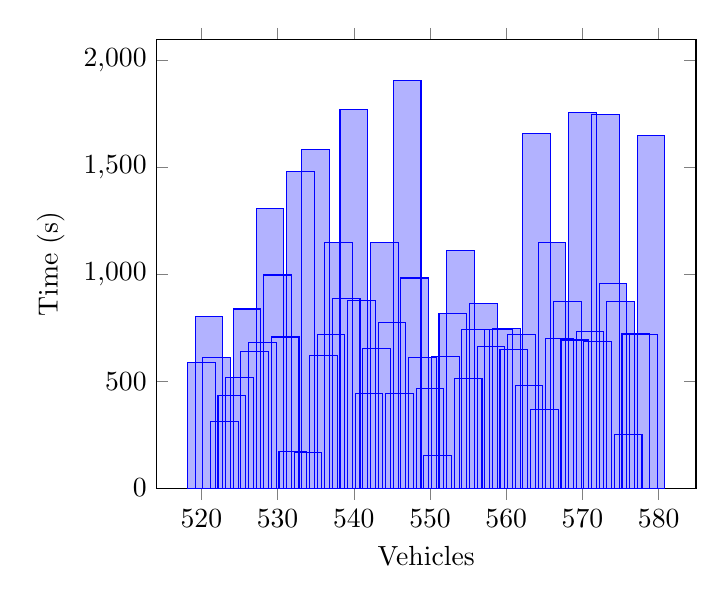
\begin{tikzpicture}
\begin{axis}[
legend style={anchor=west},
xlabel=Vehicles,
ylabel=Time (s),
ymin=0,
ybar,
]
\addplot coordinates {
(561, 649)
(557, 863)
(573, 1749)
(541, 877)
(558, 661)
(559, 740)
(522, 609)
(533, 1481)
(530, 997)
(528, 681)
(542, 444)
(527, 637)
(546, 444)
(569, 693)
(553, 818)
(534, 165)
(545, 774)
(574, 959)
(539, 887)
(543, 655)
(552, 615)
(525, 519)
(520, 588)
(544, 1148)
(536, 622)
(547, 1907)
(548, 983)
(550, 468)
(554, 1113)
(551, 151)
(571, 733)
(523, 312)
(549, 613)
(576, 249)
(531, 707)
(538, 1150)
(540, 1770)
(579, 1650)
(567, 698)
(526, 838)
(562, 717)
(521, 802)
(555, 513)
(524, 435)
(575, 873)
(556, 742)
(529, 1310)
(564, 1657)
(570, 1758)
(532, 173)
(537, 719)
(535, 1585)
(568, 874)
(566, 1149)
(578, 718)
(560, 747)
(563, 480)
(577, 721)
(565, 367)
(572, 686)
};

\end{axis}
\end{tikzpicture}
\label{tik:time:100:95}
\caption{100 percent diving with GSC on route $95$}
\end{figure}
